\documentclass{article}
\usepackage[utf8]{inputenc}
\usepackage{siunitx}
\usepackage{graphics}
\usepackage[american,siunitx]{circuitikz}
\usepackage{amsmath}
\usepackage{svg} 
\usepackage{booktabs}
\usepackage{float}
\usepackage{xparse, xfp}
\usepackage{graphicx} 
\usepackage{steinmetz}
\usepackage{forest}
\usepackage{adjustbox}
\usepackage{tikz}
\forestset{  default preamble={for tree={circle,draw}  }}
\renewcommand{\thesubsection}{\thesection.\alph{subsection}}
\newcommand{\equal}{=}
\ExplSyntaxOn
\NewDocumentCommand{\defcon}{mm}
 {
  \cs_new:Npx #1 { \fp_eval:n { #2 } }
 }
\ExplSyntaxOff

\title{ECE3310\\Data Structure\\\,\\Midterm\\Resubmission of Question 3, 4, 6, and 8\\}
\author{Choi Tim Antony Yung}
\date{19 March 2020}

\begin{document}

\clearpage\maketitle
\thispagestyle{empty}

\newpage
\setcounter{page}{1}

\setcounter{section}{2}
\section{}
\subsection{}
\begin{table}[H]
    \centering
    \begin{tabular}{rl}
            \toprule
            Character&Huffman Code\\
            \midrule
            A&011\\
            B&000\\
            C&001\\
            D&010\\
            E&1\\
            \bottomrule
    \end{tabular}
    \caption{Huffman Code for Tree 1}
\end{table}

\subsection{}
$EL1=0.2\times3+0.1\times3+0.1\times3+0.15\times3+0.45\times1=2.1$

\subsection{Tree 2}
\begin{forest}
    [1.0[0.55,edge label={node[midway,left,font=\scriptsize]{0}}[0.4,edge label={node[midway,left,font=\scriptsize]{0}}[0.3,edge label={node[midway,left,font=\scriptsize]{0}}[0.2,tier=char,edge label={node[midway,left,font=\scriptsize]{0}},draw]{\draw () node[anchor=south,label={[label distance=-1.25cm]A}]{};}[0.1,tier=char,edge label={node[midway,right,font=\scriptsize]{1}},draw]{\draw () node[anchor=south,label={[label distance=-1.25cm]B}]{};}][0.1,tier=char,edge label={node[midway,right,font=\scriptsize]{1}},draw]{\draw () node[anchor=south,label={[label distance=-1.25cm]C}]{};}][0.15,tier=char,edge label={node[midway,right,font=\scriptsize]{1}},draw]{\draw () node[anchor=south,label={[label distance=-1.25cm]D}]{};}][0.45,edge label={node[midway,right,font=\scriptsize]{1}},tier=char,draw]{\draw () node[anchor=south,label={[label distance=-1.25cm]E}]{};}]
\end{forest}

\subsection{}
\begin{table}[H]
    \centering
    \begin{tabular}{rl}
            \toprule
            Character&Huffman Code\\
            \midrule
            A&0000\\
            B&0001\\
            C&001\\
            D&01\\
            E&1\\
            \bottomrule
    \end{tabular}
    \caption{Huffman Code for Tree 2}
\end{table}

\subsection{}
$EL2=0.2\times4+0.1\times4+0.1\times3+0.15\times2+0.45\times1=2.25$

\subsection{}
EL1 do not agree with EL2. The length for the characters differs for different tree built with the same character and frequency, as the configuration of the characters changes between different trees, the reduction of length to node of higher frequency character would skew EL to a lower value and vice versa, therefore it is reasonable that EL1 does not necessarily agree with EL2 as the increase in length to A with frequency 0.2 and the increase in length to B and C skewed EL to a higher value that cannot be offset by the reduction in length to D.

\section{}
\subsection{FCFS}
\begin{adjustbox}{max width=\textwidth}
  \begin{tikzpicture}
    % draw horizontal line   
    \draw (0,0) -- (27,0);

    % draw vertical lines
    \foreach \x in {0,5,8,16,22,27}
      \draw (\x cm,10pt) -- (\x cm,-10pt);

    % draw nodes
    \draw (0,0) node[below=10pt] {\huge$ 0 $} node[above=10pt] {\huge$   $};
    \draw (5,0) node[below=10pt] {\huge$ 5 $} node[above=10pt] {\huge$   $};
    \draw (8,0) node[below=10pt] {\huge$ 8 $} node[above=10pt] {\huge$   $};
    \draw (16,0) node[below=10pt] {\huge$ 16 $} node[above=10pt] {\huge$   $};
    \draw (22,0) node[below=10pt] {\huge$ 22 $} node[above=10pt] {\huge$   $};
    \draw (27,0) node[below=10pt] {\huge$ 27 $} node[above=10pt] {\huge$   $};
    
    \draw (2.5,0) node[below=10pt] {\huge$  $} node[above=10pt] {\huge P0};
    \draw (6.5,0) node[below=10pt] {\huge$  $} node[above=10pt] {\huge P1};
    \draw (12,0) node[below=10pt] {\huge$  $} node[above=10pt] {\huge P2};
    \draw (19,0) node[below=10pt] {\huge$  $} node[above=10pt] {\huge P3};
    \draw (24.5,0) node[below=10pt] {\huge$  $} node[above=10pt] {\huge P4};
    
  \end{tikzpicture}
\end{adjustbox}
\begin{table}[H]
    \centering
    \begin{tabular}{r|ccc|c}
            \toprule
            Process&Arrival&Execution&Service&Wait\\
            &Time&Time&Time&Time\\
            \midrule
            P0&0&5&0&$0-0=0$\\
            P1&1&3&5&$5-1=4$\\
            P2&2&8&8&$8-2=6$\\
            P3&3&6&16&$16-3=13$\\
            P4&4&5&22&$22-4=18$\\
            \bottomrule
    \end{tabular}
\end{table}

\subsection{SJN}
\begin{adjustbox}{max width=\textwidth}
  \begin{tikzpicture}
    % draw horizontal line   
    \draw (0,0) -- (27,0);

    % draw vertical lines
    \foreach \x in {0,5,8,13,19,27}
      \draw (\x cm,10pt) -- (\x cm,-10pt);

    % draw nodes
    \draw (0,0) node[below=10pt] {\huge$ 0 $} node[above=10pt] {\huge$   $};
    \draw (5,0) node[below=10pt] {\huge$ 5 $} node[above=10pt] {\huge$   $};
    \draw (8,0) node[below=10pt] {\huge$ 8 $} node[above=10pt] {\huge$   $};
    \draw (13,0) node[below=10pt] {\huge$ 13 $} node[above=10pt] {\huge$   $};
    \draw (19,0) node[below=10pt] {\huge$ 19 $} node[above=10pt] {\huge$   $};
    \draw (27,0) node[below=10pt] {\huge$ 27 $} node[above=10pt] {\huge$   $};
    
    \draw (2.5,0) node[below=10pt] {\huge$  $} node[above=10pt] {\huge P0};
    \draw (6.5,0) node[below=10pt] {\huge$  $} node[above=10pt] {\huge P1};
    \draw (10.5,0) node[below=10pt] {\huge$  $} node[above=10pt] {\huge P4};
    \draw (16,0) node[below=10pt] {\huge$  $} node[above=10pt] {\huge P3};
    \draw (23,0) node[below=10pt] {\huge$  $} node[above=10pt] {\huge P2};
    
  \end{tikzpicture}
\end{adjustbox}
\begin{table}[H]
    \centering
    \begin{tabular}{r|ccc|c}
            \toprule
            Process&Arrival&Execution&Service&Wait\\
            &Time&Time&Time&Time\\
            \midrule
            P0&0&5&0&$0-0=0$\\
            P1&1&3&5&$5-1=4$\\
            P2&2&8&19&$19-2=17$\\
            P3&3&6&13&$13-3=10$\\
            P4&4&5&8&$8-4=4$\\
            \bottomrule
    \end{tabular}
\end{table}

\subsection{Priority Scheduling}
\begin{adjustbox}{max width=\textwidth}
  \begin{tikzpicture}
    % draw horizontal line   
    \draw (0,0) -- (27,0);

    % draw vertical lines
    \foreach \x in {0,5,10,16,19,27}
      \draw (\x cm,10pt) -- (\x cm,-10pt);

    % draw nodes
    \draw (0,0) node[below=10pt] {\huge$ 0 $} node[above=10pt] {\huge$   $};
    \draw (5,0) node[below=10pt] {\huge$ 5 $} node[above=10pt] {\huge$   $};
    \draw (10,0) node[below=10pt] {\huge$ 10 $} node[above=10pt] {\huge$   $};
    \draw (16,0) node[below=10pt] {\huge$ 16 $} node[above=10pt] {\huge$   $};
    \draw (19,0) node[below=10pt] {\huge$ 19 $} node[above=10pt] {\huge$   $};
    \draw (27,0) node[below=10pt] {\huge$ 27 $} node[above=10pt] {\huge$   $};
    
    \draw (2.5,0) node[below=10pt] {\huge$  $} node[above=10pt] {\huge P0};
    \draw (7.5,0) node[below=10pt] {\huge$  $} node[above=10pt] {\huge P4};
    \draw (13,0) node[below=10pt] {\huge$  $} node[above=10pt] {\huge P3};
    \draw (17.5,0) node[below=10pt] {\huge$  $} node[above=10pt] {\huge P1};
    \draw (23,0) node[below=10pt] {\huge$  $} node[above=10pt] {\huge P2};
    
  \end{tikzpicture}
\end{adjustbox}
\begin{table}[H]
    \centering
    \begin{tabular}{r|cccc|c}
            \toprule
            Process&Arrival&Execution&Priority&Service&Wait\\
            &Time&Time&&Time&Time\\
            \midrule
            P0&0&5&1&0&$0-0=0$\\
            P1&1&3&2&16&$16-1=15$\\
            P2&2&8&1&19&$19-2=17$\\
            P3&3&6&3&10&$10-3=7$\\
            P4&4&5&4&5&$5-4=1$\\
            \bottomrule
    \end{tabular}
\end{table}

\subsection{Shortest Remaining Time}
\begin{adjustbox}{max width=\textwidth}
  \begin{tikzpicture}
    % draw horizontal line   
    \draw (0,0) -- (27,0);

    % draw vertical lines
    \foreach \x in {0,1,4,8,13,19,27}
      \draw (\x cm,10pt) -- (\x cm,-10pt);

    % draw nodes
    \draw (0,0) node[below=10pt] {\huge$ 0 $} node[above=10pt] {\huge$   $};
    \draw (1,0) node[below=10pt] {\huge$ 1 $} node[above=10pt] {\huge$   $};
    \draw (4,0) node[below=10pt] {\huge$ 4 $} node[above=10pt] {\huge$   $};
    \draw (8,0) node[below=10pt] {\huge$ 8 $} node[above=10pt] {\huge$   $};
    \draw (13,0) node[below=10pt] {\huge$ 13 $} node[above=10pt] {\huge$   $};
    \draw (19,0) node[below=10pt] {\huge$ 19 $} node[above=10pt] {\huge$   $};
    \draw (27,0) node[below=10pt] {\huge$ 27 $} node[above=10pt] {\huge$   $};
    
    \draw (0.5,0) node[below=10pt] {\huge$  $} node[above=10pt] {\huge P0};
    \draw (2.5,0) node[below=10pt] {\huge$  $} node[above=10pt] {\huge P1};
    \draw (6,0) node[below=10pt] {\huge$  $} node[above=10pt] {\huge P0};
    \draw (10.5,0) node[below=10pt] {\huge$  $} node[above=10pt] {\huge P4};
    \draw (16,0) node[below=10pt] {\huge$  $} node[above=10pt] {\huge P3};
    \draw (23,0) node[below=10pt] {\huge$  $} node[above=10pt] {\huge P2};
    
  \end{tikzpicture}
\end{adjustbox}
\begin{table}[H]
    \centering
    \begin{tabular}{r|ccc|r}
            \toprule
            Process&Arrival&Execution&Service&Wait\\
            &Time&Time&Time&Time\\
            \midrule
            P0&0&5&0,4&$(0-0)+(4-1)=3$\\
            P1&1&3&1&$1-1=0$\\
            P2&2&8&19&$19-2=17$\\
            P3&3&6&13&$13-3=10$\\
            P4&4&5&8&$8-4=4$\\
            \bottomrule
    \end{tabular}
\end{table}

\subsection{Round Robin with Quantum = 3}
\begin{adjustbox}{max width=\textwidth}
  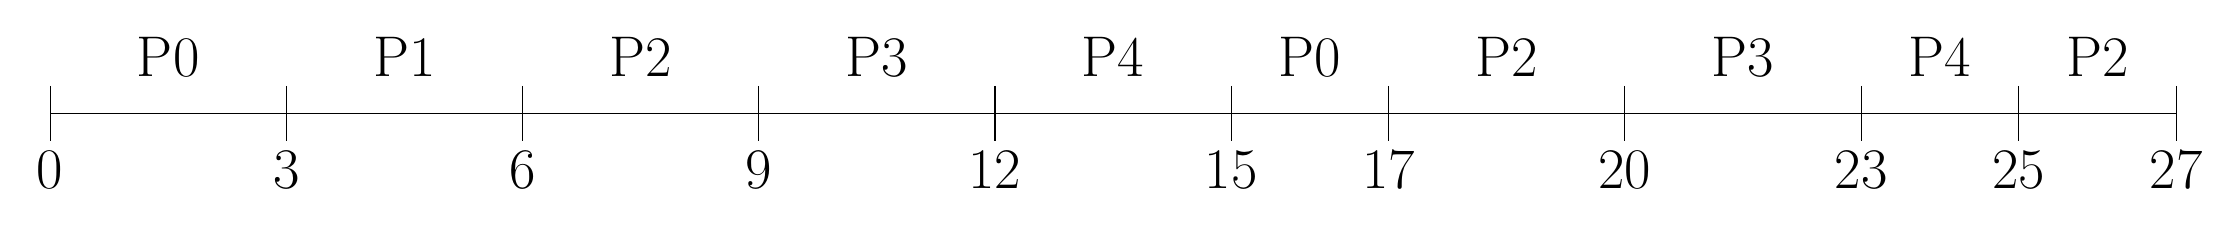
\begin{tikzpicture}
    % draw horizontal line   
    \draw (0,0) -- (27,0);

    % draw vertical lines
    \foreach \x in {0,3,6,9,12,15,17,20,23,25,27}
      \draw (\x cm,10pt) -- (\x cm,-10pt);

    % draw nodes
    \draw (0,0) node[below=10pt] {\huge$ 0 $} node[above=10pt] {\huge$   $};
    \draw (3,0) node[below=10pt] {\huge$ 3 $} node[above=10pt] {\huge$   $};
    \draw (6,0) node[below=10pt] {\huge$ 6 $} node[above=10pt] {\huge$   $};
    \draw (9,0) node[below=10pt] {\huge$ 9 $} node[above=10pt] {\huge$   $};
    \draw (12,0) node[below=10pt] {\huge$ 12 $} node[above=10pt] {\huge$   $};
    \draw (15,0) node[below=10pt] {\huge$ 15 $} node[above=10pt] {\huge$   $};
    \draw (17,0) node[below=10pt] {\huge$ 17 $} node[above=10pt] {\huge$   $};
    \draw (20,0) node[below=10pt] {\huge$ 20 $} node[above=10pt] {\huge$   $};
    \draw (23,0) node[below=10pt] {\huge$ 23 $} node[above=10pt] {\huge$   $};
    \draw (25,0) node[below=10pt] {\huge$ 25 $} node[above=10pt] {\huge$   $};
    \draw (27,0) node[below=10pt] {\huge$ 27 $} node[above=10pt] {\huge$   $};
    
    \draw (1.5,0) node[below=10pt] {\huge$  $} node[above=10pt] {\huge P0};
    \draw (4.5,0) node[below=10pt] {\huge$  $} node[above=10pt] {\huge P1};
    \draw (7.5,0) node[below=10pt] {\huge$  $} node[above=10pt] {\huge P2};
    \draw (10.5,0) node[below=10pt] {\huge$  $} node[above=10pt] {\huge P3};
    \draw (13.5,0) node[below=10pt] {\huge$  $} node[above=10pt] {\huge P4};
    \draw (16,0) node[below=10pt] {\huge$  $} node[above=10pt] {\huge P0};
    \draw (18.5,0) node[below=10pt] {\huge$  $} node[above=10pt] {\huge P2};
    \draw (21.5,0) node[below=10pt] {\huge$  $} node[above=10pt] {\huge P3};
    \draw (24,0) node[below=10pt] {\huge$  $} node[above=10pt] {\huge P4};
    \draw (26,0) node[below=10pt] {\huge$  $} node[above=10pt] {\huge P2};
    
  \end{tikzpicture}
\end{adjustbox}
\begin{table}[H]
    \centering
    \begin{tabular}{r|ccc|r}
            \toprule
            Process&Arrival&Execution&Service&Wait\\
            &Time&Time&Time&Time\\
            \midrule
            P0&0&5&0,15&$(0-0)+(15-3)=12$\\
            P1&1&3&3&$3-1=2$\\
            P2&2&8&6,17,25&$(6-2)+(17-9)+(25-20)=17$\\
            P3&3&6&9,20&$(9-3)+(20-12)=14$\\
            P4&4&5&12,23&$(12-5)+(23-15)=15$\\
            \bottomrule
    \end{tabular}
\end{table}

\subsection{Round Robin with Quantum = 2}
\begin{adjustbox}{max width=\textwidth}
  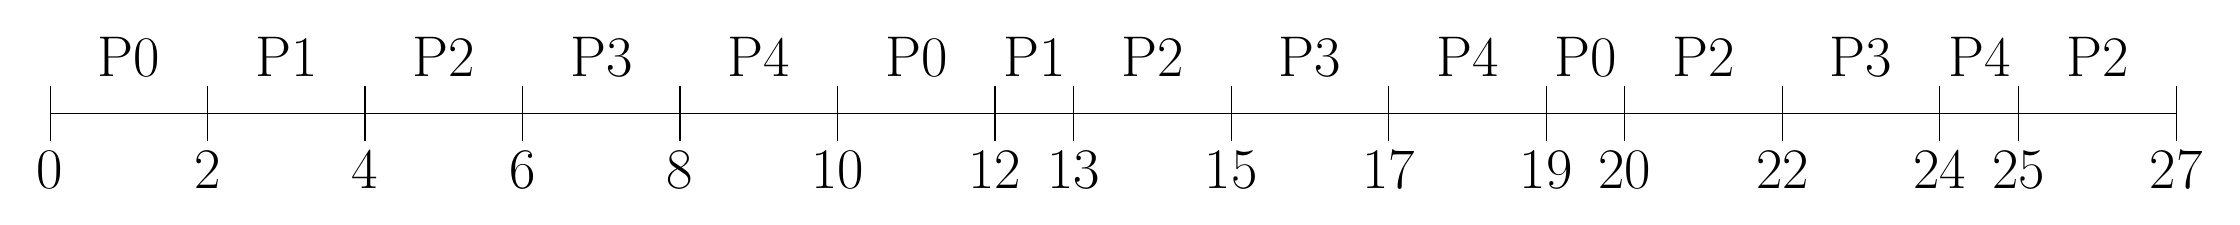
\begin{tikzpicture}
    % draw horizontal line   
    \draw (0,0) -- (27,0);

    % draw vertical lines
    \foreach \x in {0,2,4,6,8,10,12,13,15,17,19,20,22,24,25,27}
      \draw (\x cm,10pt) -- (\x cm,-10pt);

    % draw nodes
    \draw (0,0) node[below=10pt] {\huge$ 0 $} node[above=10pt] {\huge$   $};
    \draw (2,0) node[below=10pt] {\huge$ 2 $} node[above=10pt] {\huge$   $};
    \draw (4,0) node[below=10pt] {\huge$ 4 $} node[above=10pt] {\huge$   $};
    \draw (6,0) node[below=10pt] {\huge$ 6 $} node[above=10pt] {\huge$   $};
    \draw (8,0) node[below=10pt] {\huge$ 8 $} node[above=10pt] {\huge$   $};
    \draw (10,0) node[below=10pt] {\huge$ 10 $} node[above=10pt] {\huge$   $};
    \draw (12,0) node[below=10pt] {\huge$ 12 $} node[above=10pt] {\huge$   $};
    \draw (13,0) node[below=10pt] {\huge$ 13 $} node[above=10pt] {\huge$   $};
    \draw (15,0) node[below=10pt] {\huge$ 15 $} node[above=10pt] {\huge$   $};
    \draw (17,0) node[below=10pt] {\huge$ 17 $} node[above=10pt] {\huge$   $};
    \draw (19,0) node[below=10pt] {\huge$ 19 $} node[above=10pt] {\huge$   $};
    \draw (20,0) node[below=10pt] {\huge$ 20 $} node[above=10pt] {\huge$   $};
    \draw (22,0) node[below=10pt] {\huge$ 22 $} node[above=10pt] {\huge$   $};
    \draw (24,0) node[below=10pt] {\huge$ 24 $} node[above=10pt] {\huge$   $};
    \draw (25,0) node[below=10pt] {\huge$ 25 $} node[above=10pt] {\huge$   $};
    \draw (27,0) node[below=10pt] {\huge$ 27 $} node[above=10pt] {\huge$   $};
    
    \draw (1,0) node[below=10pt] {\huge$  $} node[above=10pt] {\huge P0};
    \draw (3,0) node[below=10pt] {\huge$  $} node[above=10pt] {\huge P1};
    \draw (5,0) node[below=10pt] {\huge$  $} node[above=10pt] {\huge P2};
    \draw (7,0) node[below=10pt] {\huge$  $} node[above=10pt] {\huge P3};
    \draw (9,0) node[below=10pt] {\huge$  $} node[above=10pt] {\huge P4};
    \draw (11,0) node[below=10pt] {\huge$  $} node[above=10pt] {\huge P0};
    \draw (12.5,0) node[below=10pt] {\huge$  $} node[above=10pt] {\huge P1};
    \draw (14,0) node[below=10pt] {\huge$  $} node[above=10pt] {\huge P2};
    \draw (16,0) node[below=10pt] {\huge$  $} node[above=10pt] {\huge P3};
    \draw (18,0) node[below=10pt] {\huge$  $} node[above=10pt] {\huge P4};
    \draw (19.5,0) node[below=10pt] {\huge$  $} node[above=10pt] {\huge P0};
    \draw (21,0) node[below=10pt] {\huge$  $} node[above=10pt] {\huge P2};
    \draw (23,0) node[below=10pt] {\huge$  $} node[above=10pt] {\huge P3};
    \draw (24.5,0) node[below=10pt] {\huge$  $} node[above=10pt] {\huge P4};
    \draw (26,0) node[below=10pt] {\huge$  $} node[above=10pt] {\huge P2};
    
  \end{tikzpicture}
\end{adjustbox}
\begin{table}[H]
    \centering
        \resizebox{\columnwidth}{!}{%
    \begin{tabular}{r|ccc|r}
            \toprule
            Process&Arrival&Execution&Service&Wait\\
            &Time&Time&Time&Time\\
            \midrule
            P0&0&5&0,10,19&$(0-0)+(10-2)+(19-12)=15$\\
            P1&1&3&2,12&$(2-1)+(12-4)=9$\\
            P2&2&8&4,13,20,25&$(4-2)+(13-6)+(20-15)+(25-22)=17$\\
            P3&3&6&6,15,22&$(6-3)+(15-8)+(22-17)=15$\\
            P4&4&5&8,17,24&$(8-4)+(17-10)+(24-19)=16$\\
            \bottomrule
    \end{tabular}}
\end{table}

\setcounter{section}{5}
\section{}
\subsection{}
As n-bytes signed type uses one bit for the sign, 8n bits is used to represents $2^{8n-1}$ negative values, 1 zero and $2^{8n-1}-1$ positive values. Therefore int, a signed 4 bytes range from $-(2^{(4Bytes\times8bits)-1})=2^{31}=-2147483648$ to $2^{(4Bytes\times8bit)-1}-1=2^{31}-1=2147483647$
\subsection{}
The maximum of a single precision is when sign bit is 0 (positive), the 8 bits exponent is at its maximum ($254-127=127$ as defined in IEEE 754) and the 23 bits mantissa at its maximum (all bits as 1). The maximum number can then be calculated as follow: $$(1+\sum_{i=1}^{23}\frac{1}{2^i})\times2^{127}=3.4028234663852885981170418348451692544\times10^{38}$$
The minimum would be almost the same except with the sign bit being 1:
$$-3.4028234663852885981170418348451692544\times10^{38}$$
The minimum (denormal) positive number is when both the exponent ($1-127=-126$) and mantissa ($2^{-23}$) is at its minimum, the value is then:
$$2^{-126}\times2^{-23}=2^{-149}\approx1.4013\times10^{-45}$$
The mantissa increments at a value of $2^{-23}\approx10^{-7}$, which means it can provide 7 digits of precision.
\subsection{}
As n-bytes signed type uses one bit for the sign, 8n bits is used to represents $2^{8n-1}$ negative values, 1 zero and $2^{8n-1}-1$ positive values. Therefore long, a signed 8 bytes range from $-(2^{(8Bytes\times8bits)-1})=2^{63}=-9223372036854775808$ to $2^{(8Bytes\times8bits)-1}-1=2^{63}-1=9223372036854775807$
\subsection{}
The maximum of a double precision is when sign bit is 0 (positive), the 11 bits exponent is at its maximum ($2046-1023=1023$ as defined in IEEE 754) and the 52 bits mantissa at its maximum (all bits as 1). The maximum number can then be calculated as follow: $$(1+\sum_{i=1}^{52}\frac{1}{2^i})\times2^{1023}\approx1.79769\times10^{308}$$
The minimum would be almost the same except with the sign bit being 1:
$$\approx-1.79769\times10^{308}$$
The minimum (denormal) positive number is when both the exponent ($1-1023=-1022$) and mantissa ($2^{-52}$) is at its minimum, the value is then:
$$2^{-1022}\times2^{-52}=2^{-1076}\approx4.941\times10^{-324}$$
The mantissa increments at a value of $2^{-52}\approx2\times10^{-16}$, which means it can provide around 16 digits of precision.

\setcounter{section}{7}
\section{}
\subsection{}
The maximum of a quadruple precision is when sign bit is 0 (positive), the 15 bits exponent is at its maximum ($32766-16383=16383$ as defined in IEEE 754) and the 112 bits mantissa at its maximum (all bits as 1). The maximum number can then be calculated as follow: $$(1+\sum_{i=1}^{112}\frac{1}{2^i})\times2^{16383}\approx1.1897\times10^{4932}$$
The minimum would be almost the same except with the sign bit being 1:
$$\approx-1.1897\times10^{4932}$$
The minimum (denormal) positive number is when both the exponent ($1-16383=-16382$) and mantissa ($2^{-112}$) is at its minimum, the value is then:
$$2^{-16382}\times2^{-112}=2^{-16494}\approx6.475175\times10^{-4966}$$
The mantissa increments at a value of $2^{-112}\approx2\times10^{-34}$, which means it can provide around 34 digits of precision.
\subsection{}
The maximum of an octuple precision is when sign bit is 0 (positive), the 19 bits exponent is at its maximum ($524286-262143=262143$ as defined in IEEE 754) and the 236 bits mantissa at its maximum (all bits as 1). The maximum number can then be calculated as follow: $$(1+\sum_{i=1}^{236}\frac{1}{2^i})\times2^{262143}\approx1.6113257175\times10^{78913}$$
The minimum would be almost the same except with the sign bit being 1:
$$\approx-1.6113257175\times10^{78913}$$
The minimum (denormal) positive number is when both the exponent ($1-262143=-262142$) and mantissa ($2^{-236}$) is at its minimum, the value is then:
$$2^{-262142}\times2^{-236}=2^{-262378}\approx2.248\times 10^{-78984}$$
The mantissa increments at a value of $2^{-236}\approx10^{-73}$, which means it can provide around 73 digits of precision.
\subsection{}
In report 1 the following values of $50!$ was obtained using different tools:
\begin{table}[H]
    \centering
    \begin{tabular}{rl}
            \toprule
            Tools&Value of $50!$\\
            \midrule
            Excel&3.04141E+64\\
            MATLAB&3.041409320171338e+64\\
            Calculator&3.0414093201713378043612608166065e+64\\
            \bottomrule
    \end{tabular}
\end{table}
As Calculator have the most number of digits of $50!$, it seems to be the case that it have the highest precision (32 decimal digits $\approx$ quadruple precision). However, as it only have half the number of decimal digits precision as octuple precision, it is unlikely that calculator, and other tools that have lower precision than it, have the same or higher than octuple precision.

\end{document}

